\chapter{Estado de la Cuestión}
\label{cap:estadoDeLaCuestion}

En este capítulo, se estudiarán detalladamente las simulaciones basadas en agentes de inteligencia artificial y modelos de lenguaje, así como las complejidades en las relaciones sociales y la interacción persona-ordenador. El objetivo fundamental es contextualizar la evolución histórica y actual de estos temas, destacando la relevancia de su estudio y desarrollo, subrayando la importancia de que estos sistemas puedan ser fácilmente extensibles y utilizados por profesionales de distintos ámbitos. El capítulo se dividirá en varios puntos, los cuales se pueden englobar en dos secciones.

La primera sección del estado de la cuestión se centra en las simulaciones basadas en agentes y su aplicación en entornos de inteligencia artificial. Se explorarán los avances tecnológicos, las metodologías y los desarrollos más recientes que han influido en la creación de sistemas de simulación avanzados. Asimismo, se examinará la relación de estos agentes con modelos de lenguaje, identificando los desafíos de esta convergencia tecnológica.

Después, se revisarán los desarrollos más destacados en procesamiento del lenguaje natural (PLN) y cómo estos contribuyen a la mejora de la interacción entre humanos y sistemas de inteligencia artificial. Además, se explorarán los aspectos psicológicos relacionados con las relaciones sociales en el contexto de la informática. También se centrará en la interacción persona-ordenador, se analizarán las tendencias actuales en diseño centrado en el usuario y las estrategias para garantizar que las simulaciones de inteligencia artificial sean accesibles a todos los públicos, independientemente de su desconocimiento sobre la tecnología.

\section{Simulaciones basadas en agentes}
\section{Modelos de lenguaje}
\subsection{Generativos}
\subsection{LLM}
\section{Agentes}

\section{Procesamiento del lenguaje natural}

El procesamiento del lenguaje natural (PLN) es una rama de la inteligencia artificial que se enfoca en la interacción entre las computadoras y el lenguaje humano. El objetivo del PLN es permitir que las máquinas comprendan y procesen el lenguaje humano de la misma manera que lo hacemos los seres humanos. Esto lo consiguen combinando la lingüística computacional con modelos estadísticos de machine learning y deep learning, pudiendo así interpretar tanto datos de texto como de voz, e incluso imágenes u otros tipos.

\subsection{Historia del PLN}

Se podría considerar el 1950 como el año de surgimiento del PLN, con la publicación de \cite{10.1093/mind/LIX.236.433}, donde se proponía el conocido \textit{Test de Turing}, una herramienta que evalúa la capacidad de una máquina para exhibir un comportamiento inteligente similar o indistinguible al de un ser humano, teniendo a una persona como evaluadora del comportamiento y comparando las respuestas con las de un humano real. Esto abrió el debate sobre si las máquinas eran o no capaces de "pensar" y sobre cómo pueden interpretar el texto que reciben y devolver una salida que cobre sentido.

Entre finales de los años 70 y el año 1985, surgieron modelos que se basaban en reglas para realizar traducciones automáticas, ya que en la época, era el principal objetivo del PLN, como Syntra \citep{Toma1970SYSTRANMT}. A principios del siglo XXI se vio que estos sistemas no eran los más eficientes y, a partir de los años 2010, s empezó a emplear el método de la inteligencia artificial para el procesamiento del lenguaje natural.

En la actualidad, las investigaciones en PLN se centran en mejorar la capacidad de las máquinas para comprender el contexto y la intención detrás del lenguaje humano. Avances notables incluyen el desarrollo de modelos de lenguaje preentrenados, como BERT (Bidirectional Encoder Representations from Transformers) y GPT (Generative Pre-trained Transformer), que han demostrado una capacidad excepcional para captar la complejidad del lenguaje natural \citep{devlin2019bert}.

A día de hoy, estos sistemas han sido perfeccionados y se utilizan de manera habitual en varios ámbitos como pueden ser la recuperación y extracción de información, la minería de datos, la traducción automática, el análisis de sentimientos o la generación de resúmenes automáticos \citep{hernandez2013aplicaciones}. En el caso de este estudio, es especialmente interesante la generación de resúmenes automáticos, ya que es una de las extensiones propuestas en los objetivos de realización del trabajo.

\subsection{PLN para resúmenes de textos}

En los últimos años, se han propuesto diversos generadores de secuencias. En particular, los que más éxito han tenido son los basados en arquitecturas de aprendizaje profundo (deep learning) \citep{mishra2020deep}. Las definiciones de la figura \ref{fig:resumenTextos} se refieren a los distintos tipos de resúmenes de textos que pueden existir, según \cite{adhikari2020nlp}. 

\begin{figure}[h]
	\centering
	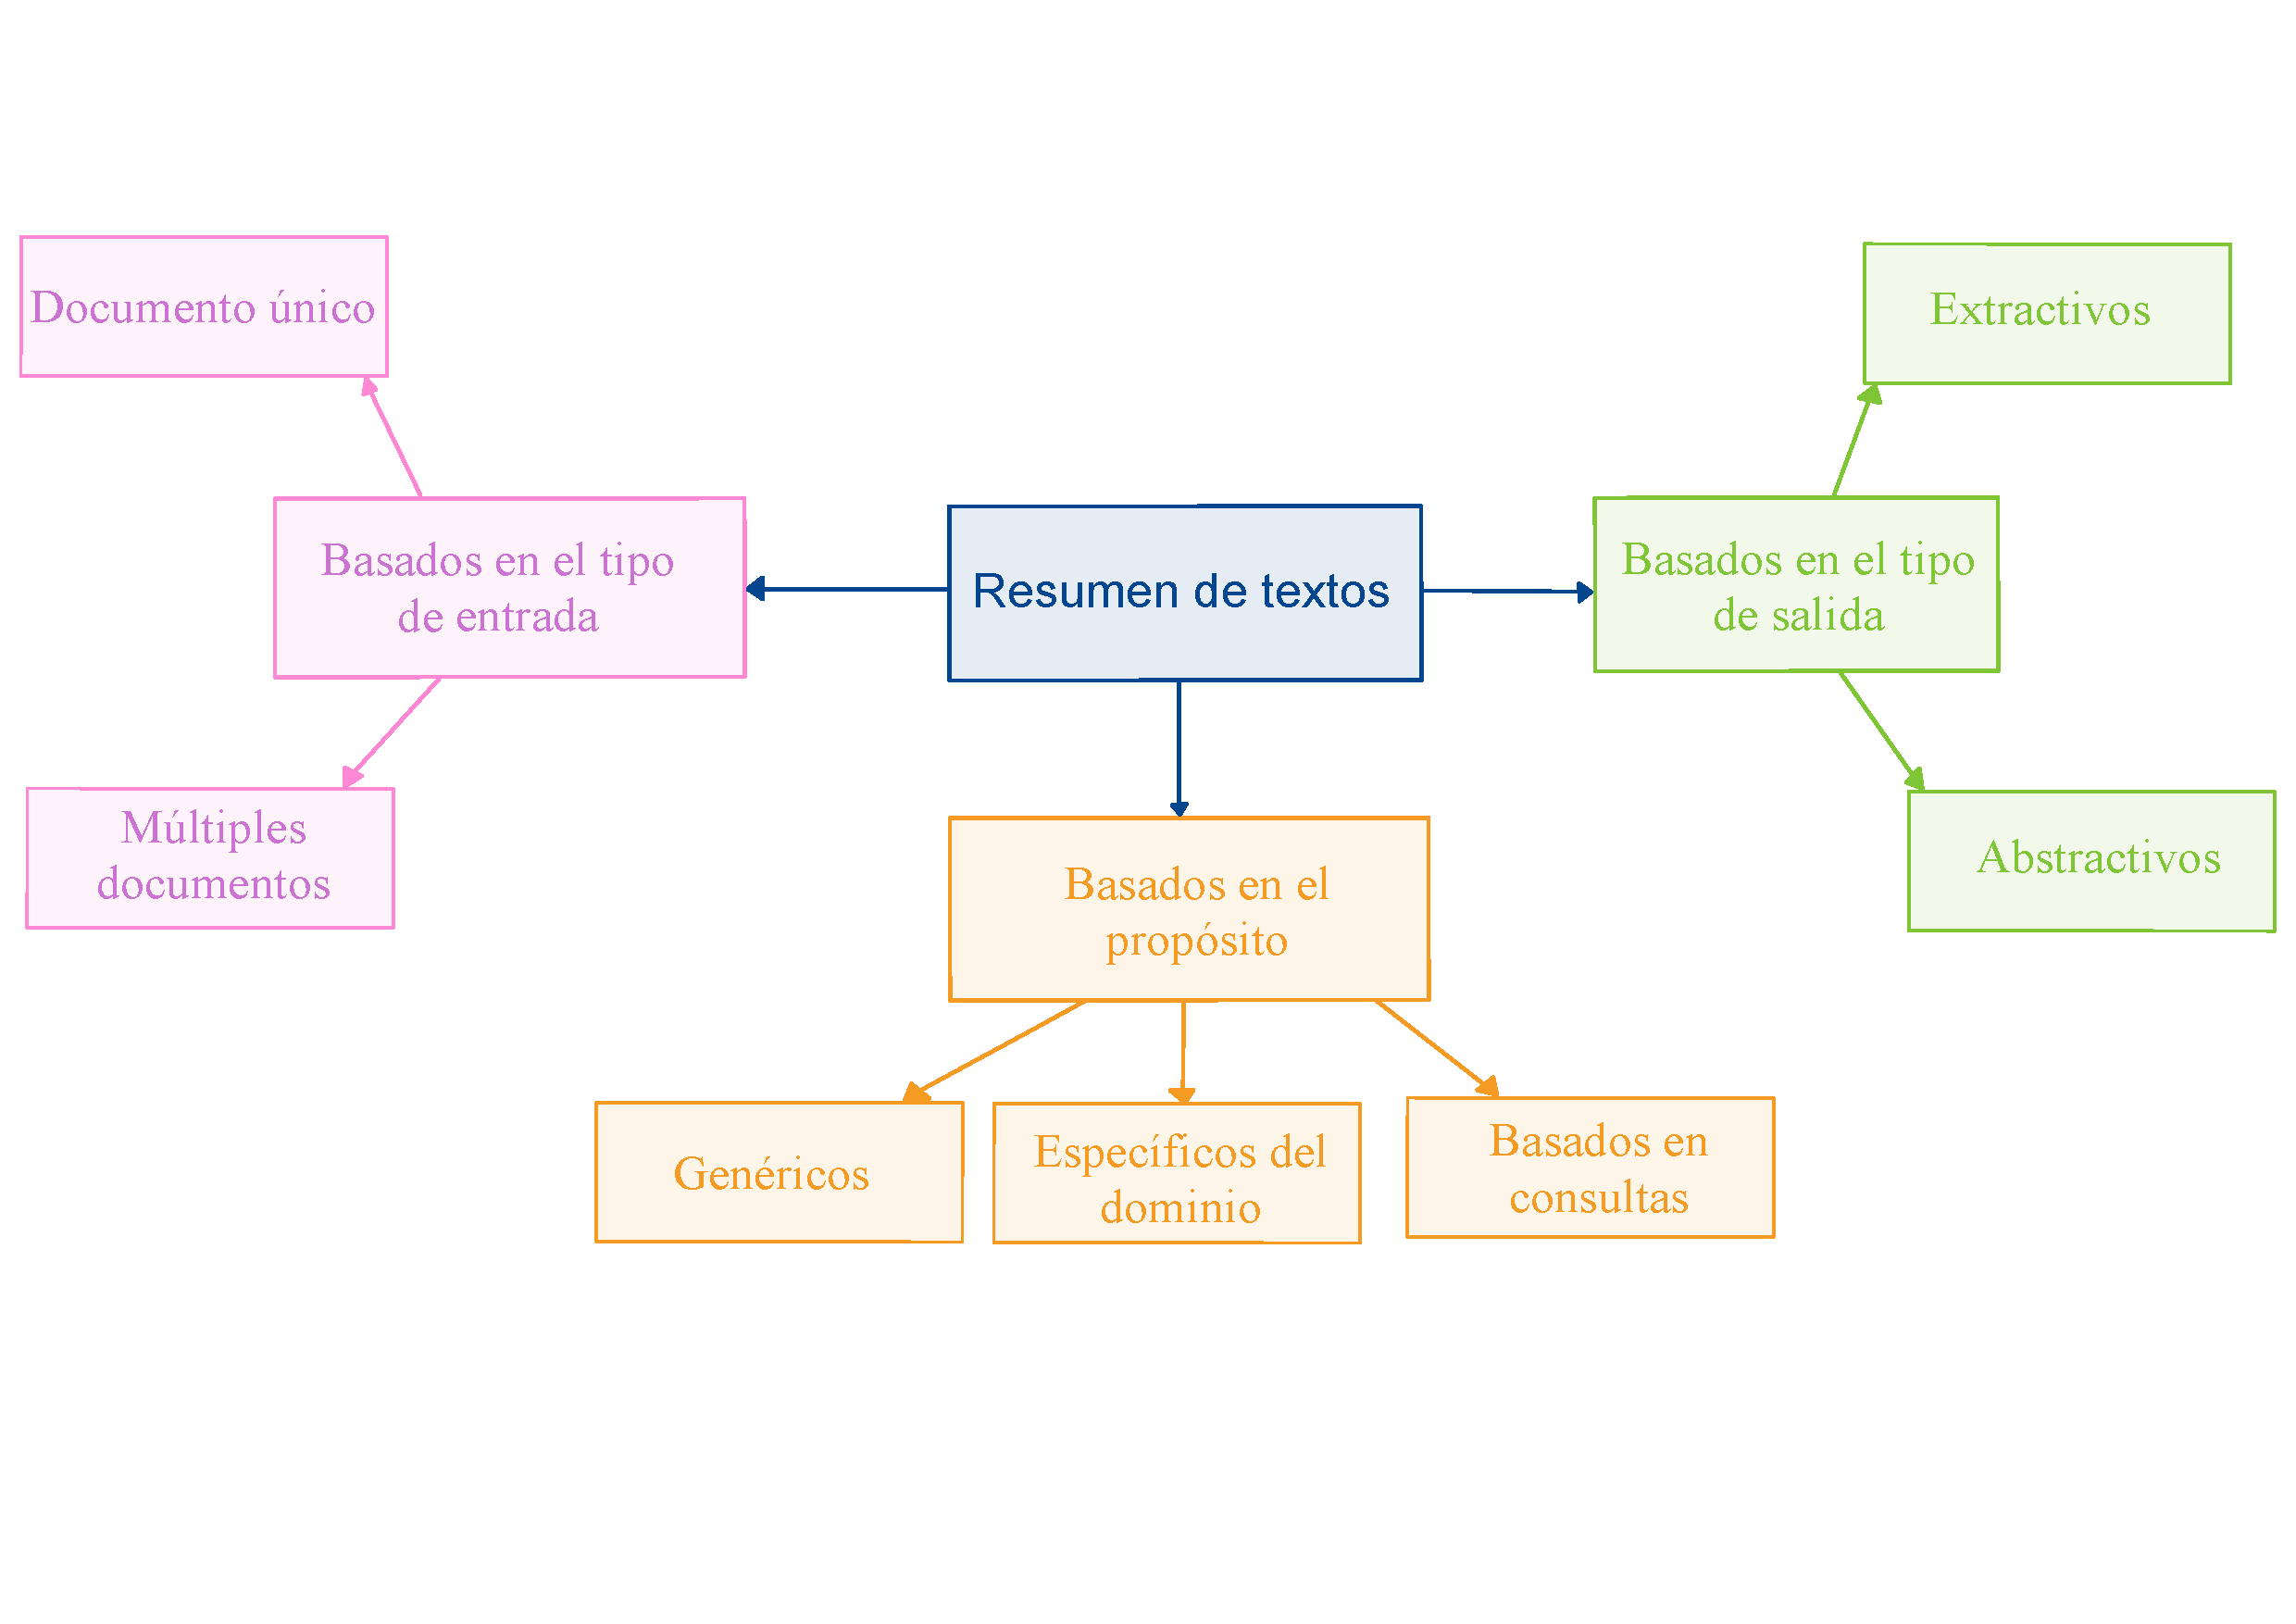
\includegraphics[width = 0.7\textwidth]{Imagenes/Vectorial/resumenTextos.pdf}
	\caption{Resumen de textos (adaptada de \cite{adhikari2020nlp})}
	\label{fig:resumenTextos}
\end{figure}

Los resúmenes extractivos son los que reutilizan las mismas frases existentes en el documento original, los abstractivos son más generales y se centran en los aspectos clave. De manera similar, las técnicas de resumen de un solo documento proporcionan resúmenes del texto de un solo documento, y las de múltiples documentos, generan resúmenes de varios documentos. Además, en la actualidad, hay una necesidad de resumir texto basándose en consultas. Los modelos de resumen basados en consultas proporcionan resúmenes del texto según un área específica descrita por la consulta proporcionada por el usuario, mientras que los resúmenes genéricos son en su mayoría resúmenes abstractos que se centran en el área general del texto de entrada.

\subsection{Impacto del desarrollo del PLN en la sociedad actual}

Como se ha visto, el procesamiento del lenguaje natural se ha desarrollado enormemente desde su concepción, especialmente en los últimos años. Con el uso de las tecnologías más modernas, se ha conseguido que el PLN sea parte del día a día de una persona común, lo cual ha traido múltiples beneficios a la sociedad, como pueden ser los siguientes:

\begin{itemize}
	\item \textbf{Mejora en la comunicación}: Facilitando la interacción con dispositivos electrónicos, como pueden ser los asistentes virtuales conocidos como Siri (de Apple) o Alexa (de Amazon). Además, al interpretar el lenguaje natural, se han creado diferentes dispositivos que permiten a personas con discapacidades, comunicarse con otra gente.
	
	\item \textbf{Progreso de la traducción automática}: Como se ha visto, la traducción automática tanto de discursos como de textos ha sido uno de los puntos de estudio principales relacionados con el PLN. A día de hoy, este ámbito está bastante desarrollado y permite unir personas de diferentes culturas y países.
	
	\item \textbf{Ayudas de soporte para negocios}: Con la proliferación de los conocidos 'chatbots', muchos negocios de todos los tamaños se han visto beneficiados, pudiendo incorporarlos como una medida de soporte para los clientes.
	
	\item \textbf{Análisis avanzado de datos}: El PLN permite utilizar enormes cantidades de texto y aportar estadísticas importantes a partir de él, lo cual sería muy difícil para os humanos debido a las grandes cantidades de información. Además, estos análisis a gran escala pueden servir para analizar los sentimientos de los mensajes publicados en redes sociales, por ejemplo.
\end{itemize}

A pesar de todas estas ventajas que el procesamiento del lenguaje natural ha aportado a la sociedad, existen varios desafíos para que esta tecnología sea capaz de funcionar. Las máquinas requieren una comunicación precisa y exacta, y los humanos hablamos con ambigüedades y de forma poco precisa en el día a día. Además, para poder transcribir a texto las palabras de una persona, es necesario un uso claro y comprensible del lenguaje. Estas solo son algunas de las barreras en las que se está trabajando para poder hacer esta tecnología accesible a todo el mundo.


\section{Computación centrada en el humano}

La computación centrada en el humano (CCH) es una disciplina que se dedica a  centrar todo el desarrollo de un sistema informátivo en los seres humanos que la usarán, así como estudiar los fenómenos relacionados más significativos. Para esto, la CCH incorpora en sus estudios varios factores humanos en el diseño y prácticas de la informática, como pueden ser circunstancias sociales o culturales, empleando para ello equipos multidisciplinares para resolver los desafíos, más que equipos puramente tecnológicos.

Este tema es abordado desde hace muchos años, analizando el artículo de \cite{Card1983ThePO}, vemos que estos abogan por una perspectiva que no solo se centre en la eficiencia técnica del sistema, argumentando que "un buen diseño de sistema se debe evaluar en términos de la eficacia con la cual el sistema ayuda a los usuarios a alcanzar sus metas". Lo cual subraya la importancia de no solo medir el éxito de un programa informático en términos de rendimiento, sino también en la capacidad del sistema para ser comprensible, usable y facilite las tareas del humano que lo usa.

Además, otro de los objetivos de la computación centrada en el humano es crear sistemas que sean adaptables a los requerimientos cambiantes del usuario. No es solamente hacer un sistema optimizado y usable por los humanos, sino que también se pueda amoldar a las necesidades cambiantes de los futuros usuarios.

\subsection{Interacción persona-ordenador }

Es un área más específica que la computación centrada en el humano, ya que esta se focaliza especialmente en la relación entre el sistema y el humano, y no se centra tanto en factores externos más globales.

Los ordenadores llegaron a nuestras vidas en la década de 1940, y la ciencia de la interacción entre las personas y ordenadores llegó en la década de 1980. Entonces, ¿entre 1940 y 1980 no había interacción entre personas y ordenadores? No exactamente. En aquellas épocas, los ordenadores no estaban tan masificadamente disponibles como lo están a día de hoy, por lo que solo un selecto grupo de personas podían "comunicarse" con ellos. Estas personas eran perfiles técnicos como ingenieros y científicos, por ello la interacción era muy compleja y un amplio conocimiento técnico era necesario. \citep{mackenzie2012human}.

A partir de la década de 1980, con la llegada de los ordenadores a la vida cotidiana de las personas, se comenzó a investigar acerca de cómo facilitar la accesibilidad a todos los públicos para interactuar con las máquinas.

\textbf{TODO: COMPLETAR ESTA SECCIÓN}

\subsection{Proceso de diseño centrado en el humano}

\textbf{TODO: COMPLETAR ESTA SECCIÓN}

\subsection{Computación afectiva}

La computación afectiva es el estudio y desarrollo de sistemas y dispositivos que reconocen, interpretan, procesan y simulan el afecto humano. Está muy relacionada con la computación centrada en los humanos, ya que hace especial hincapié en las emociones de los humanos al desarrollar sistemas informáticos. Esta rama de la computación se corresponde a un campo interdisciplinar que abarca tanto las ciencias de computación, psicología y ciencias cognitivas. Esta ciencia comenzó a ser analizada a partir del artículo científico publicado de \cite{picard1995computer}, en el cual se estudiaban maneras de aplicar la subjetividad humana a los computadores.

Dos de las áreas de la computación afectiva son la detección y reconocimiento de información emocional y la emoción en las máquinas. La primera área comienza con sensores que capturan datos sobre el estado físico o comportamiento de la persona, sin interpretar los datos de entrada. Estos sensores son análogos a las técnicas que utilizan los humanos para detectar las emociones en otras personas (expresiones faciales, posturas, temperatura corporal, etc.). En cuanto al área de la emoción en las máquinas, se estudia la capacidad que tienen estos computadores de convencer y simular emociones humanas. En el libro de \cite{minsky2007emotion} se propone que las emociones "no con específicamente tan diferentes de otros procesos a los que consideramos 'pensamiento'", por lo que podría ser que estas lleguen a simular sentimientos mediante un proceso de lógica.

\subsection{Ejemplos reales de CCH }

El campo de la computación, existen varios temas del mundo real a los que se puede aplicar, algunos ejemplos de esto son los siguientes:

\begin{itemize}
	\item \textbf{Solución de problemas en entornos distribuidos}: Abarcando sistemas de información basados en Internet, redes de información basadas en sensores o dispositivos de información móviles y vestibles (relojes inteligentes, por ejemplo). Todos estos sistemas han de ser diseñados considerando al humano como centro del estudio.
	
	\item \textbf{Sistemas multi-agente} que controlan y coordinan acciones para resolver problemas complejor, como es el caso en el que nos basamos para el presente trabajo, extendiendo y adaptando el sistema multi-agente desarrollado en es estudio de \cite{park2023generative}.
	
	\item \textbf{Definición de estructuras semánticas} para que la información multimedia dé soporte a entradaas y salidas de múltiples modalidades. Como se ha visto en el apartado anterior de PLN, este campo es muy importante para la accesibilidad a todos los públicos y que se está promoviendo en los avances actuales de la tecnología.
	
\end{itemize}

Además, existen casos de proyectos reales en los que se está aplicando la CHH, uno de ellos es la División de Ciencias Computacionales NASA/Ames, la cual está realizando una investigación como miembros del Proyecto Haughton-Mars para determinar, vía estudio de analogías, cómo de probable es que la vida humana sea fructífera en Marte. Uno de las investigaciones dentro de este proyecto es el desarrollo de robots que asistirán a los científicos, ayudándoles a tomar en consideración los factores humanos, de computación y del entorno para poder sobrevivir en Marte.

Otro de los ejemplos es el Centro de Computación Cognitiva Ubicua (CUbiC) de la Universidad Estatal de Arizona, el cual se basa en los principios de la CCH para desarrollar aplicaciones asistivas, rehabilitativas y de salud. Algunos ejemplos de estos desarrollos son los conocidos como 'Note-Taker', un dispositivo diseñado para ayudar a los estudiantescon poca visión a seguir las clases y tomar apuntes, o el 'VibroGlove', que reconoce las expresiones faciales mediante retroalimentación háptica para ayudar a personas con problemas visuales.

\section{Relaciones sociales}

El artículo de \cite{park2023generative} sobre el que se ha basado la realización de este trabajo de fin de grado, está muy enfocado en el estudio del comportamiento humano y las finalidades que podría tener el hecho de simular relaciones sociales entre agentes de inteligenicia artificial. Algunos de los casos de uso de este estudio podrían ser la incorporación a personajes no jugables en videojuegos o la simulación de entornos reales para ver cómo afectaría la introducción de cambios en el ambiente, tal y como se menciona en el artículo.

Sin embargo, las relaciones sociales son un tema importante en la psicología y se han estudiado desde diferentes perspectivas. En la informática, el estudio de las relaciones sociales se ha centrado en la creación de sistemas que permitan la interacción social en línea. Es por eso que se divide el estudio de las relaciones sociales en estos dos campos, abordando en cada uno el contexto, la historia e investigaciones anteriores relacionadas con las relaciones sociales desde dos ámbitos diferentes.

\subsection{Psicología}

Las relaciones sociales desempeñan un papel fundamental en la vida humana, impactando de manera significativa en el bienestar emocional y mental de las personas. El estudio de las interacciones sociales ha revelado una serie de beneficios intrínsecos que estas conexiones ofrecen a nivel psicológico y emocional.

A lo largo del tiempo ha habido estudios que muestran de manera consistente que los individuos con menor cantidad de relaciones sociales son mas propensos a fallecer en comparación con lo que tienen una vida social plena. Estos estudios han arrojado una mayor evidencia en países industrializados \citep{House1988}.

Una vez se conoció el claro vínculo entre las relaciones sociales y la salud de las personas, los científicos se centraron en explicar cómo ocurre esto. Generalmente, existen tres amplias maneras en las que las relaciones sociales influencian la salud: de comportamiento, psicosociales y fisiológicas \citep{doi:10.1177/0022146510383501}.

\begin{itemize}
	\item \textbf{Explicaciones de comportamiento}: 
	Los comportamientos relacionados con la salud abarcan una amplia gama de conductas personales que influyen en la salud, la morbilidad y la mortalidad. De hecho, los comportamientos relacionados con la salud explican aproximadamente el 40 por ciento de la mortalidad prematura, así como una morbilidad y discapacidad sustanciales en los Estados Unidos. \citep{activePolicyAttention}
	
	\item \textbf{Explicaciones psicosociales}: La investigación en diferentes disciplinas y poblaciones sugiere la posibilidad de que algunos mecanismos psicosociales influyan en como los lazos sociales promueven la salud. Diferentes estudios han observado solamente uno de estos mecanismos, pero debido a la complejidad de la interconexión de estos mecanismos, hace que no sea posible llegar a una conclusión certera a no ser que se estudien todos a la vez.
	
	\item \textbf{Explicaciones fisiológicas}: Profesionales de varios ámbitos del mundo de la salud han  contribuido al entendimiento de algunas acciones (consumo excesivo de comida, de alcohol, de tabaco...) para reducir el estrés. Además, estas acciones muchas veces están relacionadas con actividades sociales y, el hecho de relacionarse con gente que exceda el consumo de estas sustancias, puede afectar gravemente a la salud.
	
	
\end{itemize}

Se ha visto que las relaciones sociales pueden ser muy positivas para la salud; sin embargo, también se ha comprobado que las relaciones sociales de mala calidad, también pueden afectar de manera negativa en la salud de las personas. Un matrinonio con problemas de comunicación o de entendimiento se ha asociado con funciones del sistema inmune o endocrino afectadas \citep{doi:10.1177/0265407500171001}.

\subsection{Informática a lo largo del tiempo}

El estudio de las relaciones sociales en el ámbito de la informática ha abarcado una amplia gama de temas, desde la privacidad y la seguridad en línea hasta la influencia de las redes sociales en la política y la sociedad. Además, con la aparición de las inteligencias artificiales, últimamente también se ha investigado sobre el grado de independencia que puedan tener, o cómo de humanas se pueden sentir. También se especula por cómo de cerca está la humanidad de alcanzar a construir una inteligencia artificial general (AGI por sus siglas en inglés). Esta AGI tendría un razonamiento indistinguible del de un ser humano y una capacidad de cálculo de una máquina, por ello este tema del comportamiento humano es tan estudiado para el desarrollo de nuevas IAs.

Para el caso del presente trabajo, es especialmente interesante el análisis de comportamientos humanos en agentes de inteligencia artificial. Esto es un campo que se lleva considerando más de 20 años, con el estudio de \cite{CASTELFRANCHI1998157}. Ya en este estudio se trata de probar la emergencia de fenómenos sociales, así como la cooperación entre diferentes agentes (eso sí, con una tecnología muy inferior a la actual).

Años más tarde, se publica otro estudio con un propósito similar \citep{pan2007multi}. En este caso la intención era simular comportamientos humanos en la evacuación de emergencias. Esto revela un nuevo paradigma en el que se puede aplicar este tipo de estudio. Si se consiguen unos agentes independientes capaces de interrelacionarse entre sí, estos podrían adquirir ciertos roles y representar situaciones reales de cómo actuarían humanos con esas características en esas situaciones. En el caso de las evacuaciones de emergencia esto ayuda mucho ya que se podrían evitar catástrofes mayores.

En un estudio más reciente \citep{benvenuti2023artificial} se investiga sobre el modelado del comportamiento humano tras la irrupción de las inteligencias artificiales. Se explica que se necesita mayor investigación en esta área, prestando especial atención a la educación primaria. En el artículo se defiende que la educación debería pivotar y en lugar fomentar una cultura de sabiduría, se debería fomentar una cultura de la competencia. Esta es una de las maneras en las que las tecnologías informáticas modelan el comportamiento humano para adaptarse a las nuevas tecnologías.

Además de estos ejemplos en los que se estudian las relaciones sociales y comportamientos humanos relacionados con la inteligencia artificial, uno de los mayores avances de la humanidad en cuanto a la interconexión y fomento de las relaciones sociales a distancia fueron las redes sociales.

\subsubsection{Redes Sociales}

Las redes sociales se han convertido en una parte integral de la vida en línea. Estas permiten a los usuarios conectarse con amigos y familiares, compartir información y contenido, y participar en comunidades en línea. Esto favorece por tanto las relaciones sociales a distancia usando las tecnologías de la informática.

En 1997, Andrew Weinreich creó el sitio web 'SixDegrees.com', que se considera la primera red social de la historia, en la cual los usuarios podían configurar su página de perfil, crear listas de ocnexiones y enviar mensajes entre sus contactos.

\begin{figure}[h]
	\centering
	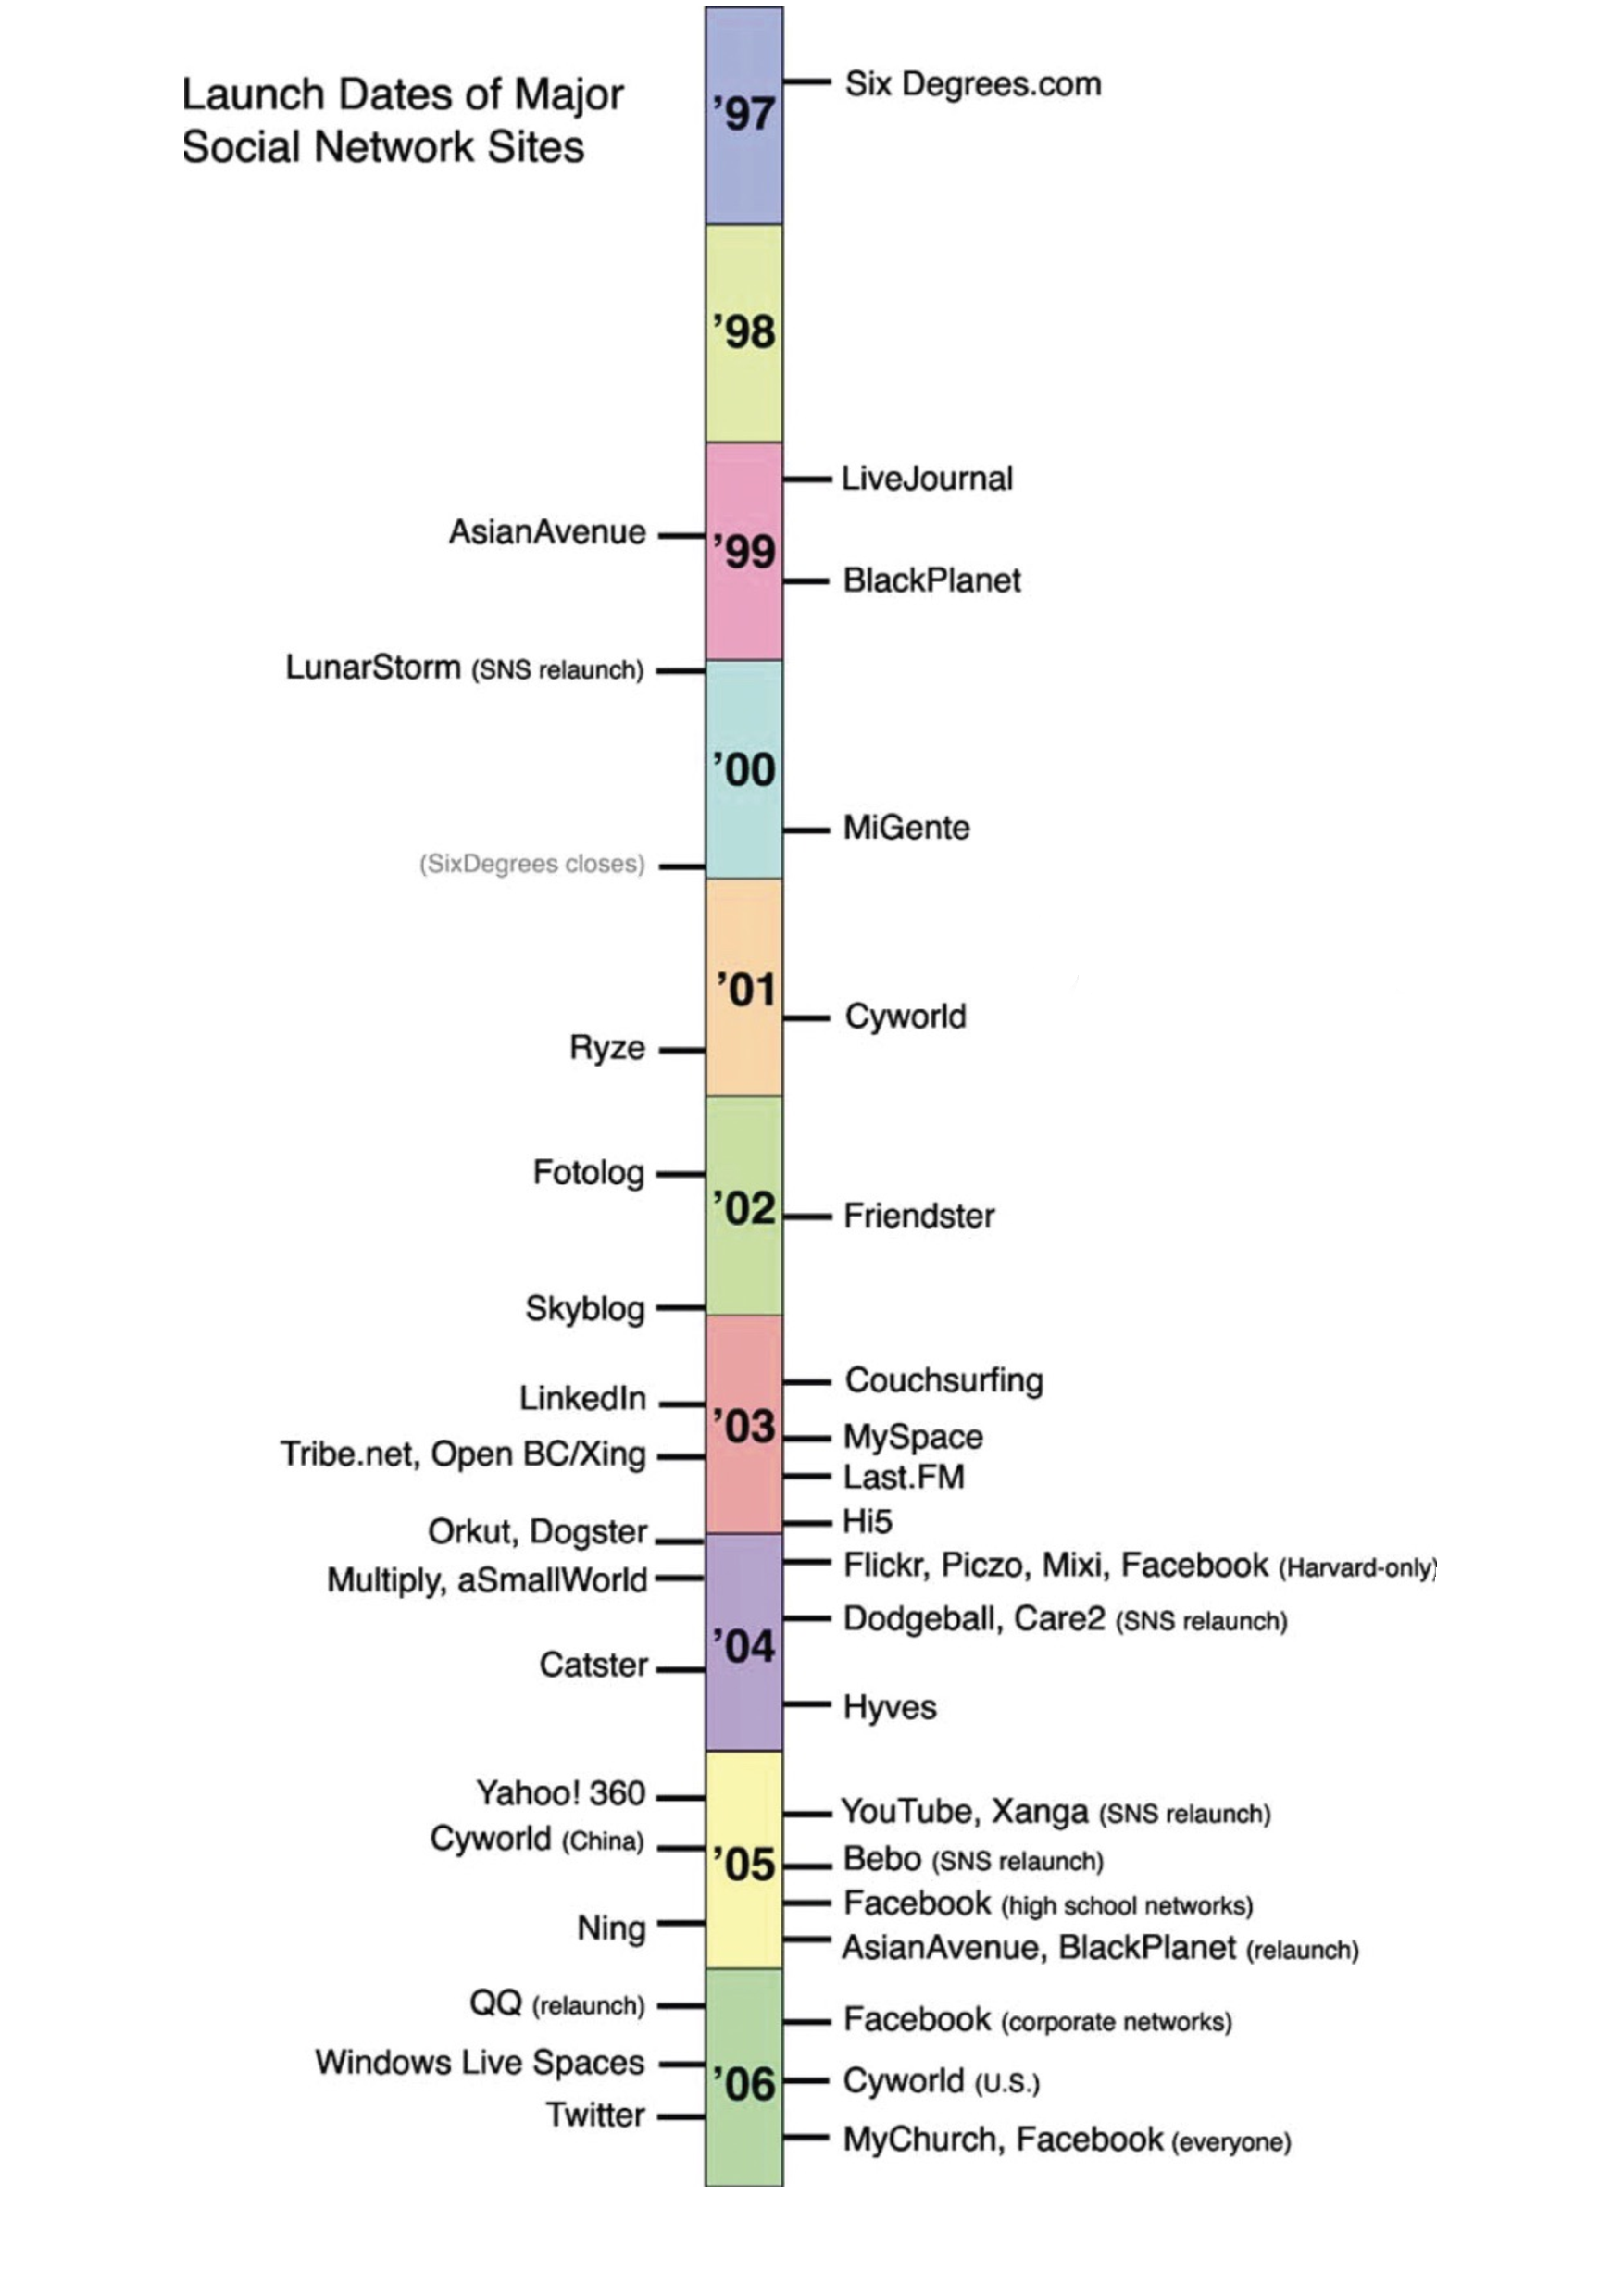
\includegraphics[width = 0.5\textwidth]{Imagenes/Vectorial/cronologiaRRSS.pdf}
	\caption{Cronología de las mayores redes sociales hasta 2006 \citep{10.1111/j.1083-6101.2007.00393.x}}
	\label{fig:cronologiaRRSS}
\end{figure}

Entre el año 1997 y el 2001, otras páginas surgieron, combinando varias funcionalidades de redes sociales como la creación de perfiles y contacto con amigos. En 2001 comenzó una nueva era para las redes sociales, con el lanzamiento de 'Ryze.com', que ayudaba a sus usuarios a incrementar sus redes de contactos empresariales.

A partir del año 2003, las redes sociales alcanzan el foco del "mainstream" y adquieren fama en todos los ámbitos, llegando a la población convencional. Es en esta época cuando comienzan a aparecer multitud de redes sociales, como 'LinkedIn' (evolución de 'Ryze.com'), 'MySpace' o 'Yahoo', algunas de ellas todavía activas a día de hoy.

Tras la explosión de estas redes en las cuales las personas se podían interconectar a distancia, se conviertió en un fenómeno global y fue escalando hasta el panorama que conocemos hoy en día. En los siguientes años se fundaron las redes sociales más populares que conocemos en la actualidad ('YouTube, 'Twitter', 'Facebook'...) y es en esta época también cuando se comienzan a crear redes sociales en torno a ciertos nichos, enfocadas para una pequeña parte de la población especialmente interesada en un tema en específico.

Los años 2010 sirvieron para que los gigantes de las redes sociales se afianzasen y las páginas más pequeñas cayesen por el camino. Además, al recibir tanto tráfico diario, estas empresas comenzaron a contratar multitud de ingenieros y diversificar sus negocios, entrando en sectores de diferente índole (Facebook comprando otras empresas como Instagram y potenciando su negocio de anuncios o Youtube siendo comprado por Google y ofreciendo múltiples formas de contenido, tanto vídeos largos o cortos como directos)

\section{Accesibilidad y extensibilidad de programas informáticos}

En el mundo actual, la accesibilidad y la extensibilidad de programas informáticos son temas cruciales. Estos conceptos no solo afectan a las personas con discapacidades, sino también a la eficiencia y la innovación en el desarrollo de software. En el caso del presente trabajo, son dos de los temas cruciales a tratar, ya que consistirá en la extensión del código ya existente en \ga, así como hacerlo más accesible para que personas con menos conocimientos técnicos también puedan emplear esta herramienta.

\subsection{Importancia de la accesibilidad}

A día de hoy, generalmente se habla de accesibilidad para referirse a la adaptación de las nuevas tecnologías para personas con discapacidad de distintos tipos. La accesibilidad en estos casos facilita la vida de las personas, mueve la inclusividad digital y amplía el alcance de las marcas, como se explica en el estudio de \citep{kavcic2005software}. Sin embargo, en este caso, se tratará el tema de la accesibilidad informática para adaptar el uso de la herramienta a perfiles no técnicos, de modo que pueda ser utilizada por gente sin conocimiento de informática y de una manera visual e intuitiva.

Promoviendo la accesibilidad para todos los públicos, se consigue que un mayor espectro de la población pueda interactuar con este tipo de herramientas, y eventualmente puedan realizar investigaciones científicas centradas en otros ámbitos. En este caso, si algún psicólogo estuviese interesado en estudiar las relaciones sociales que ocurren entre los agentes de \ga, tendría que tener ciertos conocimientos de programación para ejecutar el programa y posiblemente no lo consiguiese, democratizando el uso de la aplicación, se puede llegar a más personas y abrir distintas líneas de investigación.

\subsection{Ejemplos de accesibilidad}

\subsection{Importancia de la extensibilidad}

\subsection{Ejemplos de extensibilidad}


